%#!lualatex
\documentclass[a4j]{ltjsarticle}
\usepackage{luatexja-fontspec}
\setmainfont[Ligatures=TeX]{TeXGyreTermes}
\setsansfont[Ligatures=TeX]{TeXGyreHeros}
\setmainjfont[BoldFont=IPAexGothic]{IPAexMincho}
\setsansjfont{IPAexGothic}
\newjfontfamily\jisninety[CJKShape=JIS1990]{IPAexMincho}
\usepackage{fancyhdr,listings,url,graphicx}
%\usepackage{amsmath,amssymb,amsfonts}
\renewcommand{\ttdefault}{pcr}

\lstset{
  basicstyle=\small\ttfamily,
  keywordstyle=\bfseries,
  stringstyle=\ttfamily,
  showstringspaces=false,
  frame=tb
}
\newcommand{\dlim}{\displaystyle\lim}
\newtheorem{exercise}{演習}
\pagestyle{fancy}
\voffset=-0.5in
\textheight=720pt
\lhead{p5.js入門}
\chead{}
\rhead{}
\lfoot{}
\cfoot{\thepage}
\rfoot{}
%\renewcommand{\footrulewidth}{0.3pt}
\setlength{\columnseprule}{0.1pt}
\title{p5.js入門}
\author{数理情報研究室 濱田龍義}
\begin{document}
\maketitle
\newpage
\section{はじめに}
「情報科学」はコンピュータの初心者を対象に,コンピュータの仕組を初歩から学ぶ講義である.

大学の講義である以上,Microsoft Word や Microsoft Excel 等の
特定のソフトウェアの使い方については解説しない\footnote{学問分野ではないので,各自,自習すれば良い.ただし,この講義を受講すれば仕組を理解することによって,具体的なソフトウェアの操作についても習得しやすくなるはずである.}.
コンピュータ・サイエンスと呼ばれる学問の初歩的な部分について
p5.jsと呼ばれる\underline{プログラミング言語}を用いて学ぶ予定である.

プログラミング言語とは,人間がコンピュータに命令するための人工言語であり,
人工言語に沿って書かれた命令書自体を\underline{プログラム}と呼んだり,
命令書によって作成された実行可能な存在をプログラムと呼ぶこともある.
人工言語で書かれた命令書のことを,\underline{ソースコード}と呼ぶこともある.

また,プログラムを作成することを「プログラムする」とか,\underline{プログラミング}と呼ぶ.
p5.jsは,学んだ内容がすぐに視覚的に表現されることから,
初心者がプログラミングを学習するのに適していると言われている.

p5.jsは,Processingに影響を受けて開発されたプログラミング言語である.
ProcessingはMITメディアラボのCasey ReasとBenjamin Fryによって設計された.
電子アートとビジュアルデザインのための言語と統合開発環境から構成される.
Processingやp5.jsで作られた作品については \url{https://openprocessing.org/}
で閲覧できる.
Java言語と呼ばれるプログラミング言語を単純化し,グラッフィクに特化したものと思って良い.
最近ではアーティストだけでなくデータサイエンティスト等にも人気があり,
巨大なデータの可視化等で活躍している
%\footnote{ただし,Processing単体ではなく,C, Java, Ruby, Python, R等と組み合わせて使うことが多い}.

p5.jsはLauren McCarthyによって開発されたJavaScriptライブラリである.
JavaScriptは,Java言語と名前は似ているが別のプログラミング言語である.
現在 Python と並んで,非常に人気のあるプログラミング言語で,
テキストエディタとWebブラウザだけで試すことができる.
つまり,「メモ帳」と「Internet Explorer」だけあれば,
自宅のパソコン等でも気軽に学習を進めることができる.
講義では「TeraPad」もしくは「Atom」というテキストエディタと,「Google Chrome」を推奨する.
本稿の各ソースコードはProcessing環境を対象とした教科書
「Processingをはじめよう第2版(現題:Getting Started with Processing, Casey Reas, Ben Fry著」(船田 巧訳)と,英語の書籍``Getting Started with p5.js''(Lauren McCarthy, Casey Reas \& Ben Fry著) を参考にしている.
教科書を自分で読みながら,本稿を元にソースコードを入力し,参考にして欲しい.

\section{実習に関する注意}
\begin{enumerate}
\item 実習に関係ない私語は慎むこと.ただし,実習に関連する相談は推奨する. 
\item 自分の頭で考え,自分の手で作業を行い,自分の言葉でノートにメモを取ること.
\item 初出のキーワードはノートに書きだして確認すること.
\item 実習について,他の人のソースコードを複製してはいけない.
\item ただし,自分の手で入力したソースコードの再利用は推奨する.
\end{enumerate}

\paragraph{ソースコード入力における注意}
\begin{enumerate} 
\item 行の先頭は行番号なので入力しないこと.先頭から入力すること.
\item 括弧の対応\verb|(...)|, \verb|{...}|, カンマ \verb|, | やセミコロン \verb|;|を忘れずに入力すること.
\item コードの色分けに注意すること.
\item 大文字と小文字の区別に注意すること.
\item インデント(行頭の空白)に注意して入力すること.
\item 文字間の空白についても統一を心がけること.
%\item コンソールに表示される出力やエラーメッセージをよく読むこと.
%\item 慣れてきたら TeraPad だけでなく,Atom も試してみること.
\end{enumerate}

\section{生物資源科学部の環境について}
日本大学生物資源科学部のコンピュータ室は3つ存在する.
\begin{enumerate}
 \item 本館9階コンピュータ実習室1,
 \item 本館9階コンピュータ実習室2,
 \item 本館8階84講義室
\end{enumerate}
である.
コンピュータに関する講義,実習は基本的にこの3つの教室で行われる.
この他に,
 \begin{itemize}
  \item 本館ガレリア階,
  \item 1号館1階学生ホール,
  \item 12号館1階,
  \item 図書館
 \end{itemize}
にも自由に使えるコンピュータが用意されており,
これら7箇所のコンピュータはネットワークで接続されている.
この学内ネットワークは NUBIONET と呼ばれる.
NUBIONETに接続しているコンピュータの利用には
「NUBIONET システム利用許諾書」に書かれているユーザ名とパスワードが必要である.

NUBIONETに接続しているコンピュータでは,
ファイルサーバ\footnote{サーバとは何らかのサービスするコンピュータのこと
である.ファイルサーバの他にもメールサーバ,ウェブサーバなどが良く知られ
ている.}によって,各個人専用のファイル保存場所が用意されている.
Windows上では Z: ドライブとして表示される\footnote{自宅で参照することはできない.}.
コンピュータ室で作成し,この保存場所に保存されたファイルは,
上記7箇所のコンピュータで共有される.
ただし,インストールされているアプリケーションは,各部屋によって異なるの
で注意が必要である.詳しくは
\url{http://www.brs.nihon-u.ac.jp/it/nubionet/}
を参照すること.
%NUBIONETのユーザ名とパスワードは,実習室等のコンピュータ利用の他に,履修申請,ポータルサイトに用いられる.

一方,日本大学が全学部の学生向けに契約しているサービスとして,
NU-AppsG,Microsoft Office 365と呼ばれるものがある.
NU-AppsG (\url{https://g.nihon-u.ac.jp/})の実体は
%検索サービスやAndroid携帯で有名な
Google 社による''G Suite for Education\footnote{\url{https://gsuite.google.com/} 旧Google Apps for Education}''と呼ばれるクラウドサービス\footnote{ネットワークをベースとしたコンピュータ資源の利用方法の一種}である.
数あるサービスの中で最も重要なのがメールサービスNU-MailG''
である.学生は
\begin{lstlisting}
 brxxyyzzz@g.nihon-u.ac.jp 
\end{lstlisting}
というアドレスを用いてメールのやり取りができる.{\tt br}は BioResource
の頭文字であり,{\tt xx}は名前のイニシャル,{\tt yy}は入学年,
{\tt zzz}は学生番号の下3桁が用いられる.
このメールアドレスは大学の公式連絡手段であり,就職活動に必要なので,早いうちに慣れておくこと.
iPhoneやAndroid等のスマートフォンのメールアプリを設定して,直接読み書きすることも可能である.

\subsection{NU-AppsGについて}
%まだ,NU-MailGを利用していない方は,最初の1回だけ以下の作業が必要である.
%もし,NU-MailG のパスワードがわからないときは,コンピュータ管理室に相談すること.
%\begin{enumerate}
% \item 大学のパソコンの電源を入れる.
% \item Webブラウザ Google Chrome
%       
\includegraphics[width=7mm]{image/chrome_logo.png}を開く.
% \item 生物資源科学部のホームページ \url{http://www.brs.nihon-u.ac.jp}
%       が表示される.
% \item 下に移動し,「Webメール(在学生)」を開き,「NU-AppsG初期設定」を開く.または \url{http://g.nihon-u.ac.jp}を開く.
% \item 「アカウント通知へ」を開く.
% \item 「学生証台帳番号」,「生年月日西暦」,「確認フレーズ(画像で表示
%       されている文字)」を入力して,「次へ」をクリックする.
% \item 「学部名」「学部大学院名」「学科名」「氏名(全角カナ)」「学生番
%       号」を入力する.氏名は全角カナでスペースなしとすること.カナ小文
%       字は使えないので,カナ大文字で代用すること.学生番号は半角入力す
%       ること.
% \item 利用規約をスクロールして,最後まで読んだら「同意する」ボタンを押
%       す.
% \item 表示されるメールアドレスと,パスワードを撮影して記録しておくこと.
% \item パスワードの管理に注意すること.パスワードは変更可能である.
% \item スマートフォンで Google アカウントとして,NU-MailGのアドレスを登録すると良い.
%\end{enumerate}

%\begin{exercise}
%ネットワーク入門の履修を希望する者はWebページ
%
% \url{http://hp.brs.nihon-u.ac.jp/~hamada/nforms.html}
%
% を開き,NU-MailGのアドレス,学生番号,氏名,学科を入力すること.携帯電話でも可.
%  \begin{figure}[htbp]
%   \centering
%   \includegraphics[width=4cm]{image/net_forms.png}
%   \caption{履修登録フォーム}
%  \end{figure}
%\end{exercise}

NU-AppsG には,NU-MailG以外にも
\begin{description}
 \item[カレンダー] 予定表の作成.
 \item[ドライブ] ネットワーク上で共有できる保存領域.家と大学でファイルのやり取りが可能.
% \item[Google+] SNSサービス.
 \item[ドキュメント] ワードプロセッサの一種,文書やレポートの作成が可能,共有も可.
 \item[スプレッドシート] 表計算ソフトウェアの一種,共有も可.
 \item[スライド] プレゼンテーションソフトウェアの一種,共有も可.
 \item[サイト] Webページを簡単に作成できる.
% \item[グループ] メーリングリストや掲示板のような情報共有サービス
 \item[連絡先] アドレス帳.
 \item[YouTube] 動画サイト,動画編集や共有も可能.
 \item[マップ] 地図サービス.お気に入りの店などを保存しておくと便利.
 \item[ニュース] カスタマイズすることによって,特定のキーワードに関するニュースを表示させることも可能.
 \item[フォト] 写真保存サービス.共有も可.
 \item[翻訳] 多言語翻訳システム.最近ではカメラで撮影した他言語を翻訳することも可能.
 \item[ハングアウト] ショートメッセージ,音声通話,ビデオ通話システム.
 \item[Forms] 手軽にアンケートを作成して表計算ソフト「スプレッドシート」
	    と連携可能.
 \item[Classroom] 講義に関連したお知らせ,配布資料,課題提出などをサポートする仕組.講義でもっとも用いるサービスなのでスマートフォンにアプリをインストールしておくのも良い.
 \end{description}
など,多くのサービスが提供されている.

同じID, パスワードで Office365 と呼ばれる Microsoft 社のクラウドサービス
も利用可能である.Microsoft社の Word, Excel, PowerPoint に慣れている方は,
こちらを利用しても良い.また,Office365 アプリケーションについ
ては,1人あたり5台までプライベートパソコンやスマートフォンへの
インストールが可能である.詳しくは大学のWebページ
\url{http://www.brs.nihon-u.ac.jp/it/nubionet/software_agreement.html}
で確認できる.NU-AppsGにおけるドライブ''に相当するのがOneDrive''であ
る.こちらを用いて,家と大学でファイルを共有することもできる.

\begin{exercise}
Webブラウザ Google Chrome 
\includegraphics[width=7mm]{image/chrome_logo.png}を用いて
Google Classroom
\begin{lstlisting}
 https://classroom.google.com/
\end{lstlisting}
 を開き,タッチタイピング練習(ホームポジション基本編)を行いなさい.
なお,最初のうちは制限時間を1分に変更したほうが良い.
\end{exercise}

\begin{exercise}
Webブラウザ Google Chrome 
\includegraphics[width=7mm]{image/chrome_logo.png}を用いて
Google Classroom
\begin{lstlisting}
 https://classroom.google.com/
\end{lstlisting}
を開き,課題 Code.org 古典的迷路を20番まで解きなさい.
サービスに登録すること.「表示名」は 学生番号を半角で入力すること.
パスワードは利用しているものではなく,覚えられる新しいパスワードを設定すること.

なお,すべて緑(余計なコードが入っていると色が薄くなります.)にして終わったら,「開く」をクリックして,「完了」ボタンを押すこと.また,コメント欄に簡単なもので良いので感想を提出すること.
\end{exercise}

\begin{lstlisting}[caption=Ex\_02\_01.js]
     1: function draw() {
     2:   background(204);
     3:   ellipse(50, 50, 80, 80);
     4: }
\end{lstlisting}
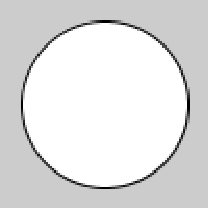
\includegraphics[height=3cm]{image/Ex_02_01.pdf}
\begin{lstlisting}[caption=Ex\_02\_02.js]
     1: function setup() {
     2:   createCanvas(480, 120);
     3: }
     4: function draw() {
     5:   if (mouseIsPressed) {
     6:     fill(0);
     7:   } else {
     8:     fill(255);
     9:   }
    10:   ellipse(mouseX, mouseY, 80, 80);
    11: }
\end{lstlisting}
マウスを動かして,円を動かしたり,クリックを試すこと.
\vspace{1in}
\begin{lstlisting}[caption=Ex\_03\_01.js]
     1: function setup() {
     2:   createCanvas(480, 120); // 教科書では 800x600 です
     3: }
     4: function draw() {
     5:   background(204);
     6: }
\end{lstlisting}
キャンバスの大きさと,背景色だけを指定.


\includegraphics[height=3cm]{image/Ex_03_01.pdf}
\begin{lstlisting}[caption=Ex\_03\_02.js]
     1: function setup() {
     2:   createCanvas(480, 120);
     3: }
     4: function draw() {
     5:   background(204);  
     6:   point(240, 60);
     7: }
\end{lstlisting}
点が1個,表示される.


\includegraphics[height=3cm]{image/Ex_03_02.pdf}
\begin{lstlisting}[caption=Ex\_03\_03.js]
     1: function setup() {
     2:   createCanvas(480, 120);
     3: }
     4: function draw() {
     5:   background(204);
     6:   line(20, 50, 420, 110);
     7: }
\end{lstlisting}
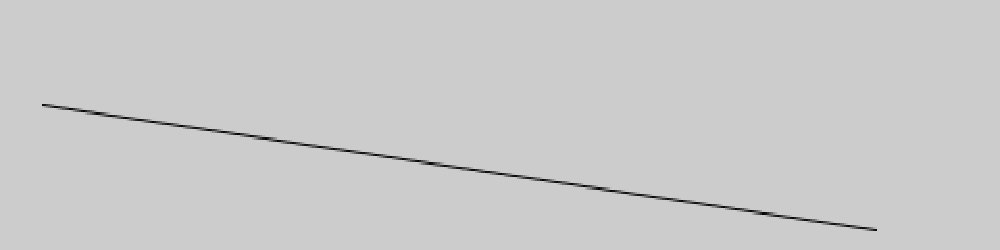
\includegraphics[height=3cm]{image/Ex_03_03.pdf}
\begin{lstlisting}[caption=Ex\_03\_04.js]
     1: function setup() {
     2:   createCanvas(480, 120);
     3: }
     4: function draw() {
     5:   background(204);
     6:   fill(255);
     7:   quad(158, 55, 199, 14, 392, 66, 351, 107);
     8:   triangle(347, 54, 392, 9, 392, 66);
     9:   triangle(158, 55, 290, 91, 290, 112);
    10: }
\end{lstlisting}

\includegraphics[height=3cm]{image/Ex_03_04.pdf}
\begin{lstlisting}[caption=Ex\_03\_05.js]
     1: function setup() {
     2:   createCanvas(480, 120);
     3: }
     4: function draw() {
     5:   background(204);
     6:   fill(255); 
     7:   rect(180, 60, 220, 40);
     8: }
\end{lstlisting}

\includegraphics[height=3cm]{image/Ex_03_05.pdf}
\begin{lstlisting}[caption=Ex\_03\_06.js]
     1: function setup() {
     2:   createCanvas(480, 120);
     3: }
     4: function draw() {
     5:   background(204);
     6:   fill(255);
     7:   ellipse(278, -100, 400, 400);
     8:   ellipse(120, 100, 110, 110);
     9:   ellipse(412, 60, 18, 18);
    10: }
\end{lstlisting}
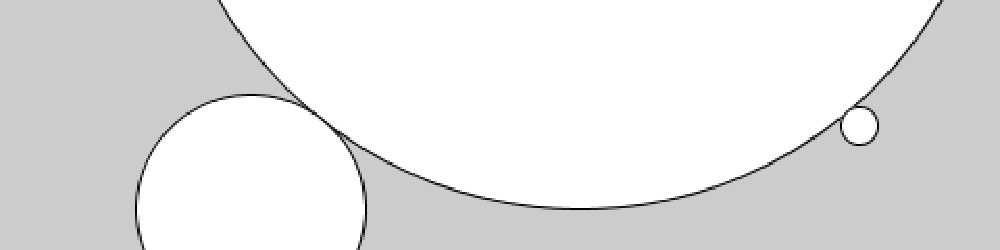
\includegraphics[height=3cm]{image/Ex_03_06.pdf}
\begin{lstlisting}[caption=Ex\_03\_07.js]
     1: function setup() {
     2:   createCanvas(480, 120);
     3: }
     4: function draw() {
     5:   background(204);
     6:   fill(255);
     7:   arc(90, 60, 80, 80, 0, HALF_PI);
     8:   arc(190, 60, 80, 80, 0, PI+HALF_PI);
     9:   arc(290, 60, 80, 80, PI, TWO_PI+HALF_PI);
    10:   arc(390, 60, 80, 80, QUARTER_PI, PI+QUARTER_PI);
    11: }
\end{lstlisting}

\includegraphics[height=3cm]{image/Ex_03_07.pdf}
\begin{lstlisting}[caption=Ex\_03\_08.js]
     1: function setup() {
     2:   createCanvas(480, 120);
     3: }
     4: function draw() {
     5:   background(204);
     6:   fill(255);
     7:   arc(90, 60, 80, 80, 0, radians(90));
     8:   arc(190, 60, 80, 80, 0, radians(270));
     9:   arc(290, 60, 80, 80, radians(180), radians(450));
    10:   arc(390, 60, 80, 80, radians(45), radians(225));
    11: }
\end{lstlisting}

\includegraphics[height=3cm]{image/Ex_03_08.pdf}
\begin{lstlisting}[caption=Ex\_03\_09.js]
     1: function setup() {
     2:   createCanvas(480, 120);
     3: }
     4: function draw() {
     5:   background(204);
     6:   fill(255);
     7:   ellipse(140, 0, 190, 190);
     8:   rect(160, 30, 260, 20);
     9: }
\end{lstlisting}
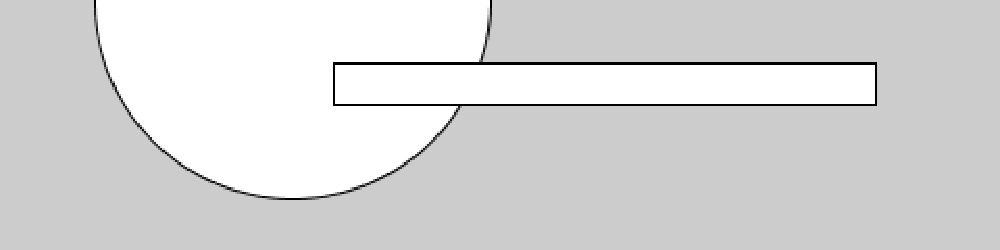
\includegraphics[height=3cm]{image/Ex_03_09.pdf}
\begin{lstlisting}[caption=Ex\_03\_10.js]
     1: function setup() {
     2:   createCanvas(480, 120);
     3: }
     4: function draw() {
     5:   background(204);
     6:   fill(255);
     7:   rect(160, 30, 260, 20);
     8:   ellipse(140, 0, 190, 190);
     9: }
\end{lstlisting}
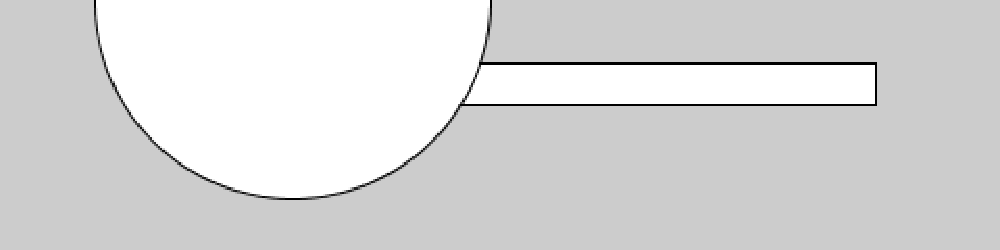
\includegraphics[height=3cm]{image/Ex_03_10.pdf}
\begin{lstlisting}[caption=Ex\_03\_11.js]
     1: function setup() {
     2:   createCanvas(480, 120);
     3:   noLoop();
     4:   background(204);
     5:   fill(255);
     6: } 
     7: function draw() {
     8:   ellipse(75, 60, 90, 90);
     9:   strokeWeight(8);
    10:   ellipse(175, 60, 90, 90);
    11:   ellipse(279, 60, 90, 90);
    12:   strokeWeight(20);
    13:   ellipse(389, 60, 90, 90);
    14: }
\end{lstlisting}
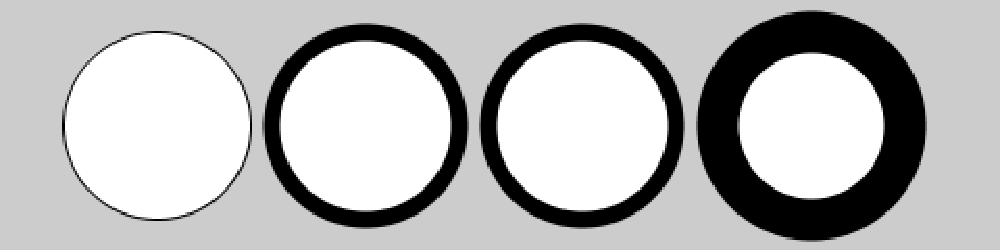
\includegraphics[height=3cm]{image/Ex_03_11.pdf}
\begin{lstlisting}[caption=Ex\_03\_12.js]
     1: function setup() {
     2:   createCanvas(480, 120);
     3:   strokeWeight(24);
     4: }
     5: function draw() {
     6:   background(204);
     7:   line(60, 25, 130, 95);
     8:   strokeCap(SQUARE);
     9:   line(160, 25, 230, 95);
    10:   strokeCap(PROJECT);
    11:   line(260, 25, 330, 95);
    12:   strokeCap(ROUND);
    13:   line(360, 25, 430, 95);
    14: }
\end{lstlisting}

\includegraphics[height=3cm]{image/Ex_03_12.pdf}
\begin{lstlisting}[caption=Ex\_03\_13.js]
     1: function setup() {
     2:   createCanvas(480, 120);
     3:   strokeWeight(12);
     4: }
     5: function draw() {
     6:   background(204);
     7:   rect(60, 25, 70, 70);
     8:   strokeJoin(ROUND);
     9:   rect(160, 25, 70, 70);
    10:   strokeJoin(BEVEL);
    11:   rect(260, 25, 70, 70);
    12:   strokeJoin(MITER);
    13:   rect(360, 25, 70, 70);
    14: }
\end{lstlisting}

\includegraphics[height=3cm]{image/Ex_03_13.pdf}
\begin{lstlisting}[caption=Ex\_03\_14.js]
     1: function setup() {
     2:   createCanvas(480, 120);
     3:   noLoop();
     4: }
     5: function draw() {
     6:   background(204);
     7:   fill(255);
     8:   rect(120, 60, 80, 80);
     9:   ellipse(120, 60, 80, 80);
    10:   ellipseMode(CORNER);
    11:   rect(280, 20, 80, 80);
    12:   ellipse(280, 20, 80, 80);
    13: }
\end{lstlisting}

\includegraphics[height=3cm]{image/Ex_03_14.pdf}
\begin{lstlisting}[caption=Ex\_03\_15.js]
     1: function setup() {
     2:   createCanvas(480, 120);
     3:   noLoop();
     4: }
     5: function draw() {
     6:   background(0);
     7:   fill(204);
     8:   ellipse(132, 82, 200, 200);
     9:   fill(153);
    10:   ellipse(228, -16, 200, 200);
    11:   fill(102);
    12:   ellipse(268, 118, 200, 200);
    13: }
\end{lstlisting}

\includegraphics[height=3cm]{image/Ex_03_15.pdf}
\begin{lstlisting}[caption=Ex\_03\_16.js]
     1: function setup() {
     2:   createCanvas(480, 120);
     3:   noLoop();
     4: }
     5: function draw() {
     6:   background(204);
     7:   fill(153);                   // Medium gray
     8:   ellipse(132, 82, 200, 200);  // Gray circle
     9:   noFill();                    // Turn off fill
    10:   ellipse(228, -16, 200, 200); // Outline circle
    11:   noStroke();                  // Turn off stroke
    12:   ellipse(268, 118, 200, 200); // Doesn’t draw!
    13: }
\end{lstlisting}

\includegraphics[height=3cm]{image/Ex_03_16.pdf}
\begin{lstlisting}[caption=Ex\_03\_17.js]
     1: function setup() {
     2:   createCanvas(480, 120);
     3:   noStroke();
     4: }
     5: function draw() {
     6:   background(0, 26, 51);       // Dark blue color
     7:   fill(255, 0, 0);             // Red color
     8:   ellipse(132, 82, 200, 200);  // Red circle
     9:   fill(0, 255, 0);             // Green color
    10:   ellipse(228, -16, 200, 200); // Green circle
    11:   fill(0, 0, 255);             // Blue color
    12:   ellipse(268, 118, 200, 200); // Blue circle
    13: }
\end{lstlisting}

\includegraphics[height=3cm]{image/Ex_03_17.pdf}
\begin{lstlisting}[caption=Ex\_03\_18.js]
     1: function setup() {
     2:   createCanvas(480, 120);
     3:   noStroke();
     4: }
     5: function draw() {
     6:   background(204, 226, 225);   // Light blue color
     7:   fill(255, 0, 0, 160);        // Red color
     8:   ellipse(132, 82, 200, 200);  // Red circle
     9:   fill(0, 255, 0, 160);        // Green color
    10:   ellipse(228, -16, 200, 200); // Green circle
    11:   fill(0, 0, 255, 160);        // Blue color
    12:   ellipse(268, 118, 200, 200); // Blue circle
    13: }
\end{lstlisting}

\includegraphics[height=3cm]{image/Ex_03_18.pdf}
\begin{lstlisting}[caption=Ex\_03\_19.js]
     1: function setup() {
     2:   createCanvas(480, 120);
     3: }
     4: function draw() {
     5:   background(204);
     6:   fill(255);
     7:   beginShape();
     8:   vertex(180, 82);
     9:   vertex(207, 36);
    10:   vertex(214, 63);
    11:   vertex(407, 11);
    12:   vertex(412, 30);
    13:   vertex(219, 82);
    14:   vertex(226, 109);
    15:   endShape();
    16: }
\end{lstlisting}

\includegraphics[height=3cm]{image/Ex_03_19.pdf}
\begin{lstlisting}[caption=Ex\_03\_20.js]
     1: function setup() {
     2:   createCanvas(480, 120);
     3: }
     4: function draw() {
     5:   background(204);
     6:   fill(255);
     7:   beginShape();
     8:   vertex(180, 82);
     9:   vertex(207, 36);
    10:   vertex(214, 63);
    11:   vertex(407, 11);
    12:   vertex(412, 30);
    13:   vertex(219, 82);
    14:   vertex(226, 109);
    15:   endShape(CLOSE);
    16: }
\end{lstlisting}

\includegraphics[height=3cm]{image/Ex_03_20.pdf}
\begin{lstlisting}[caption=Ex\_03\_21.js]
     1: function setup() {
     2:   createCanvas(480, 120);
     3: }
     4: function draw() {
     5:   background(204);
     6:   fill(255);
     7:     
     8:   // Left creature
     9:   beginShape();
    10:   vertex(50, 120);
    11:   vertex(100, 90);
    12:   vertex(110, 60);
    13:   vertex(80, 20);
    14:   vertex(210, 60);
    15:   vertex(160, 80);
    16:   vertex(200, 90);
    17:   vertex(140, 100);
    18:   vertex(130, 120);
    19:   endShape();
    20:   fill(0);
    21:   ellipse(155, 60, 8, 8);
    22:   // Right creature
    23:   fill(255);
    24:   beginShape();
    25:   vertex(370, 120);
    26:   vertex(360, 90);
    27:   vertex(290, 80);
    28:   vertex(340, 70);
    29:   vertex(280, 50);
    30:   vertex(420, 10);
    31:   vertex(390, 50);
    32:   vertex(410, 90);
    33:   vertex(460, 120);
    34:   endShape();
    35:   fill(0);
    36:   ellipse(345, 50, 10, 10);
    37: }
\end{lstlisting}
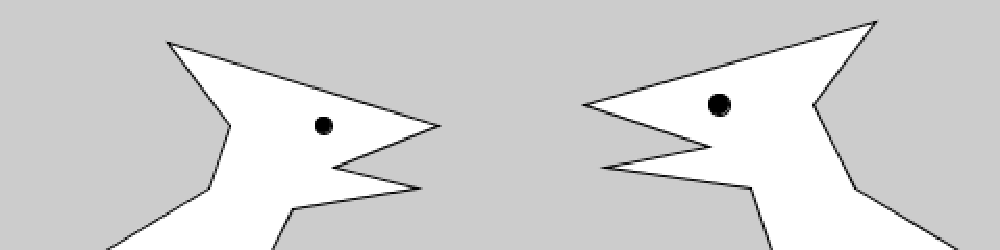
\includegraphics[height=3cm]{image/Ex_03_21.pdf}
\begin{lstlisting}[caption=Ex\_04\_01.js]
     1: var y = 60;
     2: var d = 80;
     3: function setup() {
     4:   createCanvas(480, 120);
     5: }
     6: function draw() {
     7:   background(204);
     8:   fill(255);
     9:   ellipse(75, y, d, d);   // Left
    10:   ellipse(175, y, d, d);  // Middle
    11:   ellipse(275, y, d, d);  // Right
    12: }
\end{lstlisting}

\includegraphics[height=3cm]{image/Ex_04_01.pdf}
\begin{lstlisting}[caption=Ex\_04\_02.js]
     1: var y = 100;
     2: var d = 130;
     3: function setup() {
     4:   createCanvas(480, 120);
     5: }
     6: function draw() {
     7:   background(204);
     8:   fill(255);
     9:   ellipse(75, y, d, d);   // Left
    10:   ellipse(175, y, d, d);  // Middle
    11:   ellipse(275, y, d, d);  // Right
    12: }
\end{lstlisting}

\includegraphics[height=3cm]{image/Ex_04_02.pdf}
\begin{lstlisting}[caption=Ex\_04\_03.js]
     1: function setup() {
     2:   createCanvas(480, 120);
     3: }
     4: function draw() {
     5:   background(204);
     6:   fill(255);
     7:   line(0, 0, width, height);  // Line from (0,0) to (480, 120)
     8:   line(width, 0, 0, height);  // Line from (480, 0) to (0, 120)
     9:   ellipse(width/2, height/2, 60, 60);
    10: }
\end{lstlisting}
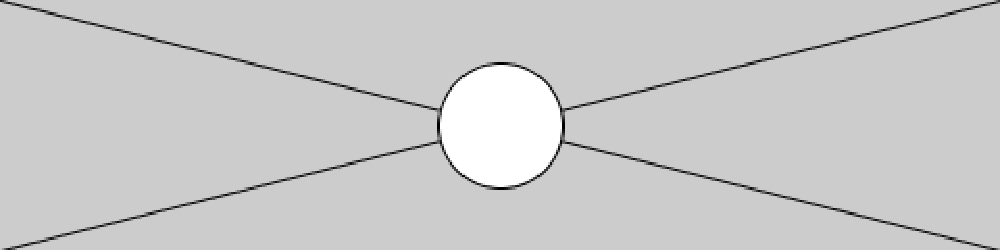
\includegraphics[height=3cm]{image/Ex_04_03.pdf}
\begin{lstlisting}[caption=Ex\_04\_04.js]
     1: var x = 25;
     2: var h = 20;
     3: var y = 25;
     4: function setup() {
     5:   createCanvas(480, 120);
     6: }
     7: function draw() {
     8:   background(204);
     9:   fill(255);
    10:   x = 20; 
    11:   rect(x, y, 300, h);       // Top
    12:   x = x + 100;
    13:   rect(x, y + h, 300, h);   // Middle
    14:   x = x - 250;
    15:   rect(x, y + h*2, 300, h); // Bottom
    16: }
\end{lstlisting}
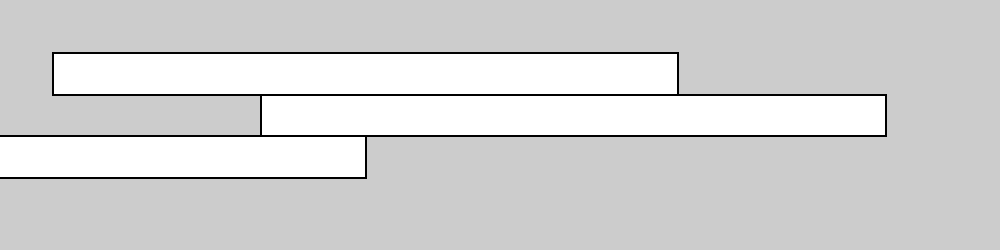
\includegraphics[height=3cm]{image/Ex_04_04.pdf}
\begin{lstlisting}[caption=Ex\_04\_05.js]
     1: function setup() {
     2:   createCanvas(480, 120);
     3:   strokeWeight(8);
     4: }
     5: function draw() {
     6:   background(204);  
     7:   line(20, 40, 80, 80);
     8:   line(80, 40, 140, 80);
     9:   line(140, 40, 200, 80);
    10:   line(200, 40, 260, 80);
    11:   line(260, 40, 320, 80);
    12:   line(320, 40, 380, 80);
    13:   line(380, 40, 440, 80);
    14: }
\end{lstlisting}

\includegraphics[height=3cm]{image/Ex_04_05.pdf}
\begin{lstlisting}[caption=Ex\_04\_06.js]
     1: function setup() {
     2:   createCanvas(480, 120);
     3:   strokeWeight(8);
     4: }
     5: function draw() {
     6:   background(204);  
     7:   for (var i = 20; i < 400; i += 60) {
     8:     line(i, 40, i + 60, 80);
     9:   }
    10: }
\end{lstlisting}

\includegraphics[height=3cm]{image/Ex_04_06.pdf}
\begin{lstlisting}[caption=Ex\_04\_07.js]
     1: function setup() {
     2:   createCanvas(480, 120);
     3:   strokeWeight(2);
     4: }
     5: function draw() {
     6:   background(204);  
     7:   for (var i = 20; i < 400; i += 8) {
     8:     line(i, 40, i + 60, 80);
     9:   }
    10: }
\end{lstlisting}

\includegraphics[height=3cm]{image/Ex_04_07.pdf}
\begin{lstlisting}[caption=Ex\_04\_08.js]
     1: function setup() {
     2:   createCanvas(480, 120);
     3:   strokeWeight(2);
     4: }
     5: function draw() {
     6:   background(204);  
     7:   for (var i = 20; i < 400; i += 20) {
     8:     line(i, 0, i + i/2, 80);
     9:   }
    10: }
\end{lstlisting}
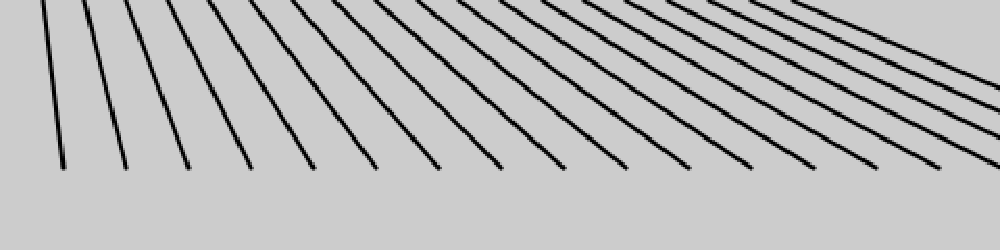
\includegraphics[height=3cm]{image/Ex_04_08.pdf}
\begin{lstlisting}[caption=Ex\_04\_09.js]
     1: function setup() {
     2:   createCanvas(480, 120);
     3:   strokeWeight(2);
     4: }
     5: function draw() {
     6:   background(204);  
     7:   for (var i = 20; i < 400; i += 20) {
     8:     line(i, 0, i + i/2, 80);
     9:     line(i + i/2, 80, i*1.2, 120);
    10:   }
    11: }
\end{lstlisting}

\includegraphics[height=3cm]{image/Ex_04_09.pdf}
\begin{lstlisting}[caption=Ex\_04\_10.js]
     1: function setup() {
     2:   createCanvas(480, 120);
     3:   noStroke();
     4: }
     5: function draw() {
     6:   background(0);
     7:   for (var y = 0; y <= height; y += 40) {
     8:     for (var x = 0; x <= width; x += 40) {
     9:       fill(255, 140);
    10:       ellipse(x, y, 40, 40);
    11:     }
    12:   }
    13: }
\end{lstlisting}

\includegraphics[height=3cm]{image/Ex_04_10.pdf}
\begin{lstlisting}[caption=Ex\_04\_11.js]
     1: function setup() {
     2:   createCanvas(480, 120);
     3:   noStroke();
     4: }
     5: function draw() {
     6:   background(0);
     7:   for (var y = 0; y < height+45; y += 40) {
     8:     fill(255, 140);
     9:     ellipse(0, y, 40, 40);
    10:   }
    11:   for (var x = 0; x < width+45; x += 40) {
    12:     fill(255, 140);
    13:     ellipse(x, 0, 40, 40);
    14:   }
    15: }
\end{lstlisting}
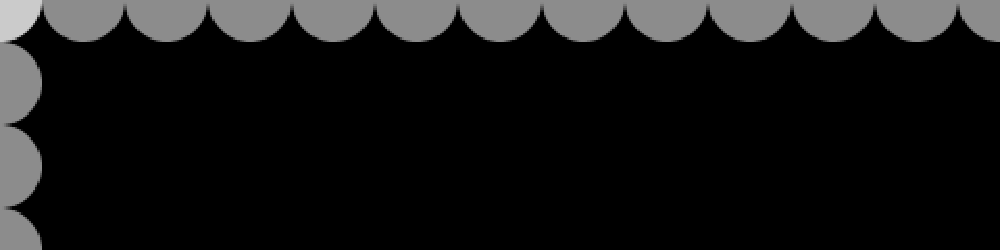
\includegraphics[height=3cm]{image/Ex_04_11.pdf}
\begin{lstlisting}[caption=Ex\_04\_12.js]
     1: function setup() {
     2:   createCanvas(480, 120);
     3:   fill(255);
     4:   stroke(102);
     5: }
     6: function draw() {
     7:   background(0);
     8:   for (var y = 20; y <= height-20; y += 10) {
     9:     for (var x = 20; x <= width-20; x += 10) {
    10:       ellipse(x, y, 4, 4);
    11:       // Draw a line to the center of the display
    12:       line(x, y, 240, 60);
    13:     }
    14:   }
    15: }
\end{lstlisting}
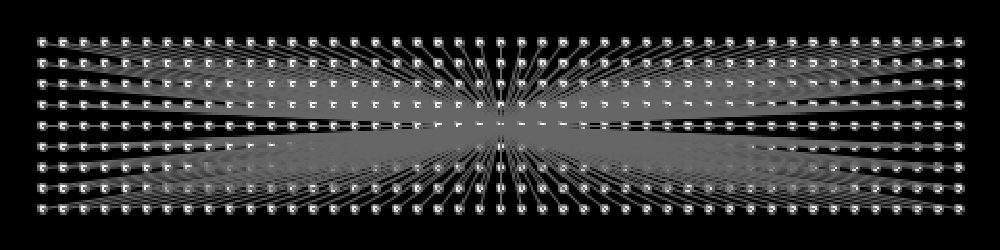
\includegraphics[height=3cm]{image/Ex_04_12.pdf}
\begin{lstlisting}[caption=Ex\_04\_13.js]
     1: function setup() {
     2:   createCanvas(480, 120);
     3: }
     4: function draw() {
     5:   background(0);
     6:   fill(255);
     7:   for (var y = 32; y <= height; y += 8) {
     8:     for (var x = 12; x <= width; x += 15) {
     9:       ellipse(x + y, y, 16 - y/10.0, 16 - y/10.0);
    10:     }
    11:   }
    12: }
\end{lstlisting}

\includegraphics[height=3cm]{image/Ex_04_13.pdf}
\begin{lstlisting}[caption=Ex\_05\_01.js]
     1: function draw() {
     2:   // Displays the frame count to the Console
     3:   print("I'm drawing");
     4:   print(frameCount);
     5: }
\end{lstlisting}
教科書を読み,どのような表示がされるか予想すること.
Google Chrome で「Ctrl + Shift + i」で Console を開く必要があります.
\vspace{1in}
\begin{lstlisting}[caption=Ex\_05\_02.js]
     1: function setup() {
     2:   print("I'm starting");
     3: }
     4: function draw() {
     5:   print("I'm running");
     6: }
\end{lstlisting}
\vspace{1in}
\begin{lstlisting}[caption=Ex\_05\_03.js]
     1: var x = 280;
     2: var y = -100;
     3: var diameter = 380;
     4: function setup() {
     5:   createCanvas(480, 120);
     6:   fill(102);
     7: }
     8: function draw() {
     9:   background(204);
    10:   ellipse(x, y, diameter, diameter);
    11: }
\end{lstlisting}
\vspace{1in}
\begin{lstlisting}[caption=Ex\_05\_04.js]
     1: function setup() {
     2:   createCanvas(480, 120);
     3:   fill(0, 102);
     4:   noStroke();
     5: }
     6: function draw() {
     7:   ellipse(mouseX, mouseY, 9, 9);
     8: }
\end{lstlisting}
\vspace{1in}
\begin{lstlisting}[caption=Ex\_05\_05.js]
     1: function setup() {
     2:   createCanvas(480, 120);
     3:   fill(0, 102);
     4:   noStroke();
     5: }
     6: function draw() {
     7:   background(204);
     8:   ellipse(mouseX, mouseY, 9, 9);
     9: }
\end{lstlisting}
\vspace{1in}
\begin{lstlisting}[caption=Ex\_05\_06.js]
     1: function setup() {
     2:   createCanvas(480, 120);
     3:   strokeWeight(4);
     4:   stroke(0, 102);
     5: }
     6: function draw() {
     7:   line(mouseX, mouseY, pmouseX, pmouseY);
     8: }
\end{lstlisting}
\vspace{1in}
\begin{lstlisting}[caption=Ex\_05\_07.js]
     1: function setup() {
     2:   createCanvas(480, 120);
     3:   stroke(0, 102);
     4: }
     5: function draw() {
     6:   var weight = dist(mouseX, mouseY, pmouseX, pmouseY);
     7:   strokeWeight(weight);
     8:   line(mouseX, mouseY, pmouseX, pmouseY);
     9: }
\end{lstlisting}
\vspace{1in}
\begin{lstlisting}[caption=Ex\_05\_08.js]
     1: var x = 0;
     2: var easing = 0.01;
     3: function setup() {
     4:   createCanvas(220, 120);
     5: }
     6: function draw() {
     7:   var targetX = mouseX;
     8:   x += (targetX - x) * easing;
     9:   ellipse(x, 40, 12, 12);
    10:   print(targetX + " : " + x);
    11: }
\end{lstlisting}
\vspace{1in}
\begin{lstlisting}[caption=Ex\_05\_09.js]
     1: var x = 0;
     2: var y = 0;
     3: var px = 0;
     4: var py = 0;
     5: var easing = 0.05;
     6: function setup() {
     7:   createCanvas(480, 120);
     8:   stroke(0, 102);
     9: }
    10: function draw() {
    11:   var targetX = mouseX;
    12:   x += (targetX - x) * easing;
    13:   var targetY = mouseY;
    14:   y += (targetY - y) * easing;
    15:   var weight = dist(x, y, px, py);
    16:   strokeWeight(weight);
    17:   line(x, y, px, py);
    18:   py = y;
    19:   px = x;
    20: }
\end{lstlisting}
\vspace{1in}
\begin{lstlisting}[caption=Ex\_05\_10.js]
     1: function setup() {
     2:   createCanvas(240, 120);
     3:   strokeWeight(30);
     4: }
     5: function draw() {
     6:   background(204);
     7:   stroke(102);
     8:   line(40, 0, 70, height);
     9:   if (mouseIsPressed == true) {
    10:     stroke(0);
    11:   }
    12:   line(0, 70, width, 50);
    13: }
\end{lstlisting}
\vspace{1in}
\begin{lstlisting}[caption=Ex\_05\_11.js]
     1: function setup() {
     2:   createCanvas(240, 120);
     3:   strokeWeight(30);
     4: }
     5: function draw() {
     6:   background(204);
     7:   stroke(102);
     8:   line(40, 0, 70, height);
     9:   if (mouseIsPressed) {
    10:     stroke(0);
    11:   } else {
    12:     stroke(255);
    13:   }
    14:   line(0, 70, width, 50);
    15: }
\end{lstlisting}
\vspace{1in}
\begin{lstlisting}[caption=Ex\_05\_12.js]
     1: function setup() {
     2:   createCanvas(120, 120);
     3:   strokeWeight(30);
     4: }
     5: function draw() {
     6:   background(204);
     7:   stroke(102);
     8:   line(40, 0, 70, height);
     9:   if (mouseIsPressed) {
    10:     if (mouseButton == LEFT) {
    11:       stroke(255);
    12:     } else {
    13:       stroke(0);
    14:     }
    15:     line(0, 70, width, 50);
    16:   }
    17: }
\end{lstlisting}
\vspace{1in}
\begin{lstlisting}[caption=Ex\_05\_13.js]
     1: var x;
     2: var offset = 10;
     3: function setup() {
     4:   createCanvas(240, 120);
     5:   x = width/2;
     6: }
     7: function draw() {
     8:   background(204);
     9:   if (mouseX > x) {
    10:     x += 0.5;
    11:     offset = -10;
    12:   }
    13:   if (mouseX < x) {
    14:     x -= 0.5;
    15:     offset = 10;
    16:   }
    17:   line(x, 0, x, height);
    18:   line(mouseX, mouseY, mouseX + offset, mouseY - 10);
    19:   line(mouseX, mouseY, mouseX + offset, mouseY + 10);
    20:   line(mouseX, mouseY, mouseX + offset*3, mouseY);
    21: }
\end{lstlisting}
\vspace{1in}
\begin{lstlisting}[caption=Ex\_05\_14.js]
     1: var x = 120;
     2: var y = 60;
     3: var radius = 12;
     4: function setup() {
     5:   createCanvas(240, 120);
     6:   ellipseMode(RADIUS);
     7: }
     8: function draw() {
     9:   background(204);
    10:   var d = dist(mouseX, mouseY, x, y);
    11:   if (d < radius) {
    12:     radius++;
    13:     fill(0);
    14:   } else {
    15:     fill(255);
    16:   }
    17:   ellipse(x, y, radius, radius);
    18: }
\end{lstlisting}
\vspace{1in}
\begin{lstlisting}[caption=Ex\_05\_15.js]
     1: var x = 80;
     2: var y = 30;
     3: var w = 80;
     4: var h = 60;
     5: function setup() {
     6:   createCanvas(240, 120);
     7: }
     8: function draw() {
     9:   background(204);
    10:   if ((mouseX > x) && (mouseX < x+w) &&
    11:     (mouseY > y) && (mouseY < y+h)) {
    12:     fill(0);
    13:   } 
    14:   else {
    15:     fill(255);
    16:   }
    17:   rect(x, y, w, h);
    18: }
\end{lstlisting}
\vspace{1in}
\begin{lstlisting}[caption=Ex\_05\_16.js]
     1: function setup() {
     2:   createCanvas(240, 120);
     3:   smooth();
     4: }
     5: function draw() {
     6:   background(204);
     7:   line(20, 20, 220, 100);
     8:   if (keyIsPressed) {
     9:     line(220, 20, 20, 100);
    10:   }
    11: }
\end{lstlisting}
\vspace{1in}
\begin{lstlisting}[caption=Ex\_05\_17.js]
     1: function setup() {
     2:   createCanvas(120, 120);
     3:   textSize(64);
     4:   textAlign(CENTER);
     5:   fill(255);    
     6: }
     7: function draw() {
     8:   background(0);  
     9:   text(key, 60, 80);
    10: }
\end{lstlisting}
\vspace{1in}
\begin{lstlisting}[caption=Ex\_05\_18.js]
     1: function setup() {
     2:   createCanvas(120, 120);
     3: }
     4: function draw() {
     5:   background(204);
     6:   if (keyIsPressed) {
     7:     if ((key == 'h') || (key == 'H')) {
     8:       line(30, 60, 90, 60);
     9:     }
    10:     if ((key == 'n') || (key == 'N')) {
    11:       line(30, 20, 90, 100);
    12:     }
    13:   }
    14:   line(30, 20, 30, 100);
    15:   line(90, 20, 90, 100);
    16: }
\end{lstlisting}
\vspace{1in}
\begin{lstlisting}[caption=Ex\_05\_19.js]
     1: var x = 215;
     2: function setup() {
     3:   createCanvas(480, 120);
     4: }
     5: function draw() {
     6:   if (keyIsPressed) {
     7:     if (keyCode == LEFT_ARROW) {
     8:       x--;
     9:     } 
    10:     else if (keyCode == RIGHT_ARROW) {
    11:       x++;
    12:     }
    13:   }
    14:   rect(x, 45, 50, 50);
    15: }
\end{lstlisting}
\vspace{1in}
\begin{lstlisting}[caption=Ex\_05\_20.js]
     1: function setup() {
     2:   createCanvas(240, 120);
     3:   strokeWeight(12);
     4: }
     5: function draw() {
     6:   background(204);
     7:   stroke(102);
     8:   line(mouseX, 0, mouseX, height);
     9:   stroke(0);
    10:   var mx = mouseX/2 + 60;
    11:   line(mx, 0, mx, height);
    12: }
\end{lstlisting}
\vspace{1in}
\begin{lstlisting}[caption=Ex\_05\_21.js]
     1: function setup() {
     2:   createCanvas(240, 120);
     3:   strokeWeight(12);
     4: }
     5: function draw() {
     6:   background(204);
     7:   stroke(102);
     8:   line(mouseX, 0, mouseX, height);
     9:   stroke(0);
    10:   var mx = map(mouseX, 0, width, 60, 180);
    11:   line(mx, 0, mx, height);
    12: }
\end{lstlisting}
\vspace{1in}
\begin{lstlisting}[caption=Ex\_06\_01.js]
     1: function setup() {
     2:   createCanvas(120, 120);
     3:   background(204);  
     4: }
     5: function draw() {
     6:   translate(mouseX, mouseY);
     7:   rect(0, 0, 30, 30);
     8: }
\end{lstlisting}
\vspace{1in}
\begin{lstlisting}[caption=Ex\_06\_02.js]
     1: function setup() {
     2:   createCanvas(120, 120); 
     3:   background(204);  
     4: }
     5: function draw() {
     6:   translate(mouseX, mouseY);
     7:   rect(0, 0, 30, 30);
     8:   translate(35, 10);
     9:   rect(0, 0, 15, 15);
    10: }
\end{lstlisting}
\vspace{1in}
\begin{lstlisting}[caption=Ex\_06\_03.js]
     1: function setup() {
     2:   createCanvas(120, 120);
     3: }
     4: function draw() {
     5:   rotate(mouseX / 100.0);
     6:   rect(0, 0, 160, 20);
     7: }
\end{lstlisting}
\vspace{1in}
\begin{lstlisting}[caption=Ex\_06\_04.js]
     1: function setup() {
     2:   createCanvas(120, 120);
     3: }
     4: function draw() {
     5:   rotate(mouseX / 100.0);
     6:   rect(-80, -10, 160, 20);
     7: }
\end{lstlisting}
\vspace{1in}
\begin{lstlisting}[caption=Ex\_06\_05.js]
     1: var angle = 0.0;
     2: function setup() {
     3:   createCanvas(120, 120);
     4:   background(204);  
     5: }
     6: function draw() {
     7:   translate(mouseX, mouseY);
     8:   rotate(angle);
     9:   rect(-15, -15, 30, 30);
    10:   angle += 0.1;
    11: }
\end{lstlisting}
\vspace{1in}
\begin{lstlisting}[caption=Ex\_06\_06.js]
     1: var angle = 0.0;
     2: function setup() {
     3:   createCanvas(120, 120);
     4:   background(204);
     5: }
     6: function draw() {
     7:   rotate(angle);
     8:   translate(mouseX, mouseY);
     9:   rect(-15, -15, 30, 30);
    10:   angle += 0.1;
    11: }
\end{lstlisting}
\vspace{1in}
\begin{lstlisting}[caption=Ex\_06\_07.js]
     1: var angle = 0.0;
     2: var angleDirection = 1;
     3: var speed = 0.005;
     4: function setup() {
     5:   createCanvas(120, 120);
     6:   //background(204);
     7: }
     8: function draw() {
     9:   background(204);
    10:   translate(20, 25);  // Move to start position
    11:   rotate(angle);
    12:   strokeWeight(12);
    13:   line(0, 0, 40, 0);
    14:   translate(40, 0);   // Move to next jovar
    15:   rotate(angle * 2.0);
    16:   strokeWeight(6);
    17:   line(0, 0, 30, 0);
    18:   translate(30, 0);   // Move the next jovar
    19:   rotate(angle * 2.5);
    20:   strokeWeight(3);
    21:   line(0, 0, 20, 0);
    22:   
    23:   angle += speed * angleDirection;
    24:   if ((angle > QUARTER_PI) || (angle < 0)) {
    25: 	angleDirection *= -1;
    26:   }
    27: }
\end{lstlisting}
\vspace{1in}
\begin{lstlisting}[caption=Ex\_06\_08.js]
     1: function setup() {
     2:   createCanvas(120, 120);
     3: }
     4: function draw() {
     5:   translate(mouseX, mouseY);
     6:   scale(mouseX / 60.0);
     7:   rect(-15, -15, 30, 30);
     8: }
\end{lstlisting}
\vspace{1in}
\begin{lstlisting}[caption=Ex\_06\_09.js]
     1: function setup() {
     2:   createCanvas(120, 120);
     3: }
     4: function draw() {
     5:   translate(mouseX, mouseY);
     6:   var scalar = mouseX / 60.0;
     7:   scale(scalar);
     8:   strokeWeight(1.0 / scalar);
     9:   rect(-15, -15, 30, 30);
    10: }
\end{lstlisting}
\vspace{1in}
\begin{lstlisting}[caption=Ex\_06\_10.js]
     1: function setup() {
     2:   createCanvas(120, 120);
     3: }
     4: function draw() {
     5:   push();
     6:   translate(mouseX, mouseY);
     7:   rect(0, 0, 30, 30);
     8:   pop();
     9:   translate(35, 10);
    10:   rect(0, 0, 15, 15);
    11: }
\end{lstlisting}
\vspace{1in}
\begin{lstlisting}[caption=Ex\_07\_01.js]
     1: var img;
     2: function preload() {
     3:   img = loadImage("media/lunar.jpg");
     4: }
     5: function setup() {
     6:   createCanvas(480, 480);
     7: }
     8: function draw() {
     9:   image(img, 0, 0);
    10: }
\end{lstlisting}
\vspace{1in}
\begin{lstlisting}[caption=Ex\_07\_02.js]
     1: var img1;
     2: var img2;
     3: function preload() {
     4:   img1 = loadImage("media/lunar.jpg");
     5:   img2 = loadImage("media/capsule.jpg");
     6: }
     7: function setup() {
     8:   createCanvas(480, 120);
     9: }
    10: function draw() {
    11:   image(img1, -120, 0);
    12:   image(img1, 130, 0, 240, 120);
    13:   image(img2, 300, 0, 240, 120);
    14: }
\end{lstlisting}
\vspace{1in}
\begin{lstlisting}[caption=Ex\_07\_03.js]
     1: var img;
     2: function preload() {
     3:   img = loadImage("media/lunar.jpg");
     4: }
     5: function setup() {
     6:   createCanvas(480, 120);
     7: }
     8: function draw() {
     9:   background(0);
    10:   image(img, 0, 0, mouseX * 2, mouseY * 2);
    11: }
\end{lstlisting}
\vspace{1in}
\begin{lstlisting}[caption=Ex\_07\_04.js]
     1: var img;
     2: function preload() {
     3:   img = loadImage("media/clouds.gif");
     4: }
     5: function setup() {
     6:   createCanvas(480, 120);
     7: }
     8: function draw() {
     9:   background(255);
    10:   image(img, 0, 0);
    11:   image(img, 0, mouseY * -1);
    12: }
\end{lstlisting}
\vspace{1in}
\begin{lstlisting}[caption=Ex\_07\_05.js]
     1: var img;
     2: function preload() {
     3:   img = loadImage("media/clouds.png");
     4: }
     5: function setup() {
     6:   createCanvas(480, 120);
     7: }
     8: function draw() {
     9:   background(204);
    10:   image(img, 0, 0);
    11:   image(img, 0, mouseY * -1);
    12: }
\end{lstlisting}
\vspace{1in}
\begin{lstlisting}[caption=Ex\_07\_06.js]
     1: function preload() {
     2:   font = loadFont("media/SourceCodePro-Regular.ttf");
     3: }
     4: function setup() {
     5:   createCanvas(480, 120);
     6:   textFont(font);
     7: }
     8: function draw() {
     9:   background(102);
    10:   fill(255);
    11:   textSize(32);
    12:   text("That's one small step for man...", 25, 60);
    13:   textSize(16);
    14:   text("That's one small step for man...", 27, 90);
    15: }
\end{lstlisting}
\vspace{1in}
\begin{lstlisting}[caption=Ex\_07\_07.js]
     1: function preload() {
     2:   font=loadFont("media/SourceCodePro-Regular.ttf");
     3: }
     4: function setup() {
     5:   createCanvas(480, 120);
     6:   textFont(font);
     7: }
     8: function draw() {
     9:   background(102);
    10:   fill(255);
    11:   textSize(22);
    12:   text("That's one small step for man...", 26, 24, 240, 100);
    13: }
\end{lstlisting}
\vspace{1in}
\begin{lstlisting}[caption=Ex\_07\_08.js]
     1: var quote = "That's one small step for man..."
     2: function preload() {
     3:   font=loadFont("media/SourceCodePro-Regular.ttf");
     4: }
     5: function setup() {
     6:   createCanvas(480, 120);
     7:   textFont(font);
     8: }
     9: function draw() {
    10:   background(102);
    11:   fill(255);
    12:   textSize(22);
    13:   text(quote, 26, 24, 240, 100);
    14: }
\end{lstlisting}
\vspace{1in}
\begin{lstlisting}[caption=Ex\_07\_09.js]
     1: var img;
     2: function preload() {
     3:   img = loadImage("media/network.svg");
     4: }
     5: function setup() {
     6:   createCanvas(480, 120);
     7: }
     8: function draw() {
     9:   background(0);
    10:   image(img, 30, 10);
    11:   image(img, 180, 10, 280, 280);
    12: }
\end{lstlisting}
\vspace{1in}
\begin{lstlisting}[caption=Ex\_07\_10.js]
     1: var img;
     2: function preload() {
     3:   img = loadImage("media/network.svg");
     4: }
     5: function setup() {
     6:   createCanvas(480, 120);
     7:   imageMode(CENTER);
     8: }
     9: function draw() {
    10:   background(0);
    11:   var diameter = map(mouseX, 0, width, 10, 800);
    12:   image(img, 120, 60, diameter, diameter);
    13: }
\end{lstlisting}
\vspace{1in}
\begin{lstlisting}[caption=Ex\_08\_01.js]
     1: function draw() {
     2:   var fr = frameRate();  
     3:   print(fr);
     4: }
\end{lstlisting}
\vspace{1in}
\begin{lstlisting}[caption=Ex\_08\_02.js]
     1: function setup() {
     2:   frameRate(30); // Thirty frames each second
     3:   //frameRate(12); // Twelve frames each second
     4:   //frameRate(2); // Two frames each second
     5:   //frameRate(0.5); // One frame every two seconds
     6: }
     7: function draw() {
     8:   var fr = frameRate();  
     9:   print(fr);
    10: }
\end{lstlisting}
\vspace{1in}
\begin{lstlisting}[caption=Ex\_08\_03.js]
     1: var radius = 40;
     2: var x = -radius;
     3: var speed = 1.5;
     4: function setup() {
     5:   createCanvas(240, 120);
     6:   ellipseMode(RADIUS);
     7: }
     8: function draw() {
     9:   background(0);
    10:   x += speed;  // Increase the value of x
    11:   arc(x, 60, radius, radius, 0.52, 5.76);
    12: }
\end{lstlisting}
\vspace{1in}
\begin{lstlisting}[caption=Ex\_08\_04.js]
     1: var radius = 40;
     2: var x = -radius;
     3: var speed = 1.5;
     4: function setup() {
     5:   createCanvas(240, 120);
     6:   ellipseMode(RADIUS);
     7: }
     8: function draw() {
     9:   background(0);
    10:   x += speed;  // Increase the value of x
    11:   if (x > width+radius) {  // If the shape is off screen
    12:     x = -radius;  // move to the left edge
    13:   }
    14:   arc(x, 60, radius, radius, 0.52, 5.76);
    15: }
\end{lstlisting}
\vspace{1in}
\begin{lstlisting}[caption=Ex\_08\_05.js]
     1: var radius = 40;
     2: var x = 110;
     3: var speed = 1.5;
     4: var direction = 1;
     5: function setup() {
     6:   createCanvas(240, 120);
     7:   ellipseMode(RADIUS);
     8: }
     9: function draw() {
    10:   background(0);
    11:   x += speed * direction;
    12:   if ((x > width-radius) || (x < radius)) {
    13:     direction = -direction; // Flip direction
    14:   }
    15:   if (direction == 1) {
    16:     arc(x, 60, radius, radius, 0.52, 5.76); // Face right
    17:   } else {
    18:     arc(x, 60, radius, radius, 3.67, 8.9); // Face left
    19:   }
    20: }
\end{lstlisting}
\vspace{1in}
\begin{lstlisting}[caption=Ex\_08\_06.js]
     1: var startX = 20;   // Initial x-coordinate
     2: var stopX = 160;   // Final x-coordinate
     3: var startY = 30;   // Initial y-coordinate
     4: var stopY = 80;    // Final y-coordinate
     5: var x = startX;    // Current x-coordinate
     6: var y = startY;    // Current y-coordinate
     7: var step = 0.005;  // Size of each step (0.0 to 1.0)
     8: var pct = 0.0;     // Percentage traveled (0.0 to 1.0)
     9: function setup() {
    10:   createCanvas(240, 120);
    11: }
    12: function draw() {
    13:   background(0);
    14:   if (pct < 1.0) {
    15:     x = startX + ((stopX-startX) * pct);
    16:     y = startY + ((stopY-startY) * pct);
    17:     pct += step;
    18:   }
    19:   ellipse(x, y, 20, 20);
    20: }
\end{lstlisting}
\vspace{1in}
\begin{lstlisting}[caption=Ex\_08\_07.js]
     1: function draw() {
     2:   var r = random(0, mouseX);
     3:   print(r);
     4: }
\end{lstlisting}
\vspace{1in}
\begin{lstlisting}[caption=Ex\_08\_08.js]
     1: function setup() {
     2:   createCanvas(240, 120);
     3: }
     4: function draw() {
     5:   background(204);
     6:   for (var x = 20; x < width; x += 20) {
     7:     var mx = mouseX / 10;
     8:     var offsetA = random(-mx, mx);
     9:     var offsetB = random(-mx, mx);
    10:     line(x + offsetA, 20, x - offsetB, 100);
    11:   }
    12: }
\end{lstlisting}
\vspace{1in}
\begin{lstlisting}[caption=Ex\_08\_09.js]
     1: var speed = 2.5;
     2: var diameter = 20;
     3: var x;
     4: var y;
     5: function setup() {
     6:   createCanvas(240, 120);
     7:   x = width/2;
     8:   y = height/2;
     9:   background(204);    
    10: }
    11: function draw() {
    12:   x += random(-speed, speed);
    13:   y += random(-speed, speed);
    14:   ellipse(x, y, diameter, diameter);
    15: }
\end{lstlisting}
\vspace{1in}
\begin{lstlisting}[caption=Ex\_08\_10.js]
     1: function draw() {
     2:   var timer = millis();
     3:   print(timer);
     4: }
\end{lstlisting}
\vspace{1in}
\begin{lstlisting}[caption=Ex\_08\_11.js]
     1: var time1 = 2000;
     2: var time2 = 4000;
     3: var x = 0;
     4: function setup() {
     5:   createCanvas(480, 120);
     6: }
     7: function draw() {
     8:   var currentTime = millis();
     9:   background(204);
    10:   if (currentTime > time2) {
    11:     x -= 0.5;
    12:   } else if (currentTime > time1) {
    13:     x += 2;
    14:   }
    15:   ellipse(x, 60, 90, 90);
    16: }
\end{lstlisting}
\vspace{1in}
\begin{lstlisting}[caption=Ex\_08\_12.js]
     1: var angle = 0.0;
     2: function draw() {
     3:   var sinval = sin(angle);
     4:   print(sinval);
     5:   var gray = map(sinval, -1, 1, 0, 255);
     6:   background(gray);
     7:   angle += 0.1;
     8: }
\end{lstlisting}
\vspace{1in}
\begin{lstlisting}[caption=Ex\_08\_13.js]
     1: var angle = 0.0;
     2: var offset = 60;
     3: var scalar = 40;
     4: var speed = 0.05;
     5: function setup() {
     6:   createCanvas(240, 120);
     7: }
     8: function draw() {
     9:   background(0);
    10:   var y1 = offset + sin(angle) * scalar;
    11:   var y2 = offset + sin(angle + 0.4) * scalar;
    12:   var y3 = offset + sin(angle + 0.8) * scalar;
    13:   ellipse( 80, y1, 40, 40);
    14:   ellipse(120, y2, 40, 40);
    15:   ellipse(160, y3, 40, 40);
    16:   angle += speed;
    17: }
\end{lstlisting}
\vspace{1in}
\begin{lstlisting}[caption=Ex\_08\_14.js]
     1: var angle = 0.0;
     2: var offset = 60;
     3: var scalar = 30;
     4: var speed = 0.05;
     5: function setup() {
     6:   createCanvas(120, 120);
     7:   background(204);
     8: }
     9: function draw() {
    10:   var x = offset + cos(angle) * scalar;
    11:   var y = offset + sin(angle) * scalar;
    12:   ellipse( x, y, 40, 40);
    13:   angle += speed;
    14: }
\end{lstlisting}
\vspace{1in}
\begin{lstlisting}[caption=Ex\_08\_15.js]
     1: var angle = 0.0;
     2: var offset = 60;
     3: var scalar = 2;
     4: var speed = 0.05;
     5: function setup() {
     6:   createCanvas(120, 120);
     7:   fill(0);
     8:   background(204);
     9: }
    10: function draw() {
    11:   var x = offset + cos(angle) * scalar;
    12:   var y = offset + sin(angle) * scalar;
    13:   ellipse( x, y, 2, 2);
    14:   angle += speed;
    15:   scalar += speed;
    16: }
\end{lstlisting}
\vspace{1in}
\begin{lstlisting}[caption=Ex\_09\_01.js]
     1: function setup() {
     2:   print("Ready to roll!");
     3:   rollDice(20);
     4:   rollDice(20);
     5:   rollDice(6);
     6:   print("Finished.");
     7: }
     8: function rollDice(numSides) {
     9:   var d = 1 + int(random(numSides));
    10:   print("Rolling... " + d);
    11: }
\end{lstlisting}
\vspace{1in}
\begin{lstlisting}[caption=Ex\_09\_02.js]
     1: function setup() {
     2:   print("Ready to roll!");
     3:   var d1 = 1 + int(random(20));
     4:   print("Rolling... " + d1);
     5:   var d2 = 1 + int(random(20));
     6:   print("Rolling... " + d2);
     7:   var d3 = 1 + int(random(6));
     8:   print("Rolling... " + d3);
     9:   print("Finished.");
    10: }
\end{lstlisting}
\vspace{1in}
\begin{lstlisting}[caption=Ex\_09\_03.js]
     1: function setup() {
     2:   createCanvas(480, 120);
     3: }
     4: function draw() {
     5:   background(204);
     6:   translate(110, 110);
     7:   stroke(0);
     8:   strokeWeight(70);
     9:   line(0, -35, 0, -65); // Body
    10:   noStroke();
    11:   fill(255);
    12:   ellipse(-17.5, -65, 35, 35);  // Left eye dome
    13:   ellipse(17.5, -65, 35, 35);   // Right eye dome
    14:   arc(0, -65, 70, 70, 0, PI);   // Chin
    15:   fill(0);
    16:   ellipse(-14, -65, 8, 8);  // Left eye
    17:   ellipse(14, -65, 8, 8);   // Right eye
    18:   quad(0, -58, 4, -51, 0, -44, -4, -51); // Beak
    19: }
\end{lstlisting}
\vspace{1in}
\begin{lstlisting}[caption=Ex\_09\_04.js]
     1: function setup() {
     2:   createCanvas(480, 120);
     3: }
     4: function draw() {
     5:   background(204);
     6:   
     7:   // Left owl
     8:   translate(110, 110);
     9:   stroke(0);
    10:   strokeWeight(70);
    11:   line(0, -35, 0, -65); // Body
    12:   noStroke();
    13:   fill(255);
    14:   ellipse(-17.5, -65, 35, 35);  // Left eye dome
    15:   ellipse(17.5, -65, 35, 35);   // Right eye dome
    16:   arc(0, -65, 70, 70, 0, PI);   // Chin
    17:   fill(0);
    18:   ellipse(-14, -65, 8, 8);  // Left eye
    19:   ellipse(14, -65, 8, 8);   // Right eye
    20:   quad(0, -58, 4, -51, 0, -44, -4, -51); // Beak
    21:   
    22:   // Right owl
    23:   translate(70, 0);
    24:   stroke(0);
    25:   strokeWeight(70);
    26:   line(0, -35, 0, -65); // Body
    27:   noStroke();
    28:   fill(255);
    29:   ellipse(-17.5, -65, 35, 35);  // Left eye dome
    30:   ellipse(17.5, -65, 35, 35);   // Right eye dome
    31:   arc(0, -65, 70, 70, 0, PI);   // Chin
    32:   fill(0);
    33:   ellipse(-14, -65, 8, 8);  // Left eye
    34:   ellipse(14, -65, 8, 8);   // Right eye
    35:   quad(0, -58, 4, -51, 0, -44, -4, -51); // Beak
    36: }
\end{lstlisting}
\vspace{1in}
\begin{lstlisting}[caption=Ex\_09\_05.js]
     1: function setup() {
     2:   createCanvas(480, 120);
     3: }
     4: function draw() {
     5:   background(204);
     6:   owl(110, 110);
     7:   owl(180, 110);
     8: }
     9: function owl(x, y) {
    10:   push();
    11:   translate(x, y);
    12:   stroke(0);
    13:   strokeWeight(70);
    14:   line(0, -35, 0, -65); // Body
    15:   noStroke();
    16:   fill(255);
    17:   ellipse(-17.5, -65, 35, 35); // Left eye dome
    18:   ellipse(17.5, -65, 35, 35);  // Right eye dome
    19:   arc(0, -65, 70, 70, 0, PI);  // Chin
    20:   fill(0);
    21:   ellipse(-14, -65, 8, 8); // Left eye
    22:   ellipse(14, -65, 8, 8);  // Right eye
    23:   quad(0, -58, 4, -51, 0, -44, -4, -51); // Beak
    24:   pop();
    25: }
\end{lstlisting}
\vspace{1in}
\begin{lstlisting}[caption=Ex\_09\_06.js]
     1: function setup() {
     2:   createCanvas(480, 120);
     3: }
     4: function draw() {
     5:   background(204);
     6:   for (var x = 35; x < width + 70; x += 70) {
     7:     owl(x, 110);
     8:   }
     9: }
    10: function owl(x, y) {
    11:   push();
    12:   translate(x, y);
    13:   stroke(0);
    14:   strokeWeight(70);
    15:   line(0, -35, 0, -65);  // Body
    16:   noStroke();
    17:   fill(255);
    18:   ellipse(-17.5, -65, 35, 35);  // Left eye dome
    19:   ellipse(17.5, -65, 35, 35);   // Right eye dome
    20:   arc(0, -65, 70, 70, 0, PI);   // Chin
    21:   fill(0);
    22:   ellipse(-14, -65, 8, 8); // Left eye
    23:   ellipse(14, -65, 8, 8);  // Right eye
    24:   quad(0, -58, 4, -51, 0, -44, -4, -51); // Beak
    25:   pop();
    26: }
\end{lstlisting}
\vspace{1in}
\begin{lstlisting}[caption=Ex\_09\_07.js]
     1: function setup() {
     2:   createCanvas(480, 120);
     3: }
     4: function draw() {
     5:   background(204);
     6:   randomSeed(0);
     7:   for (var i = 35; i < width + 40; i += 40) {
     8:     var gray = int(random(0, 102));
     9:     var scalar = random(0.25, 1.0);
    10:     owl(i, 110, gray, scalar);
    11:   }
    12: }
    13: function owl(x, y, g, s) {
    14:   push();
    15:   translate(x, y);
    16:   scale(s);  // Set the size
    17:   stroke(g); // Set the gray value
    18:   strokeWeight(70);
    19:   line(0, -35, 0, -65); // Body
    20:   noStroke();
    21:   fill(255-g);
    22:   ellipse(-17.5, -65, 35, 35); // Left eye dome
    23:   ellipse(17.5, -65, 35, 35);  // Right eye dome
    24:   arc(0, -65, 70, 70, 0, PI);  // Chin
    25:   fill(g);
    26:   ellipse(-14, -65, 8, 8);  // Left eye
    27:   ellipse(14, -65, 8, 8);   // Right eye
    28:   quad(0, -58, 4, -51, 0, -44, -4, -51); // Beak
    29:   pop();
    30: }
\end{lstlisting}
\vspace{1in}
\begin{lstlisting}[caption=Ex\_09\_08.js]
     1: function setup() {
     2:   var yourWeight = 132;
     3:   var marsWeight = calculateMars(yourWeight);
     4:   print(marsWeight);
     5: }
     6: function calculateMars(w) {
     7:   var newWeight = w * 0.38;
     8:   return newWeight;
     9: }
\end{lstlisting}
\vspace{1in}
\begin{lstlisting}[caption=Ex\_10\_01.js]
     1: var bug; // Declare object
     2: function setup() {
     3:   createCanvas(480, 120);
     4:   background(204);
     5:   fill(255);
     6:   // Create object and pass in parameters
     7:   bug = new Jitter();
     8: }
     9: function draw() {
    10:   bug.move();
    11:   bug.display();
    12: }
    13: function Jitter() {
    14:   this.x = random(width);
    15:   this.y = random(height);
    16:   this.diameter = random(10, 30);
    17:   this.speed = 2.5;
    18:   
    19:   this.move = function() {
    20:     this.x += random(-this.speed, this.speed);
    21:     this.y += random(-this.speed, this.speed);
    22:   }
    23:   
    24:   this.display = function() {
    25:     ellipse(this.x, this.y, this.diameter, this.diameter);
    26:   }
    27: }
\end{lstlisting}
\vspace{1in}
\begin{lstlisting}[caption=Ex\_10\_02.js]
     1: var jit;
     2: var bug;
     3: function setup() {
     4:   createCanvas(480, 120);
     5:   background(204);
     6:   fill(255);  
     7:   jit = new Jitter();
     8:   bug = new Jitter();
     9: }
    10: function draw() {
    11:   jit.move();
    12:   jit.display();
    13:   bug.move();
    14:   bug.display();
    15: } 
    16: function Jitter() {
    17:   this.x = random(width);
    18:   this.y = random(height);
    19:   this.diameter = random(10, 30);
    20:   this.speed = 2.5;
    21:   this.move = function() {
    22:     this.x += random(-this.speed, this.speed);
    23:     this.y += random(-this.speed, this.speed);
    24:   }
    25:   this.display = function() {
    26:     ellipse(this.x, this.y, this.diameter, this.diameter);
    27:   } 
    28: }
\end{lstlisting}
\vspace{1in}
\begin{lstlisting}[caption=Ex\_11\_01.js]
     1: var x1 = -20;
     2: var x2 = 20;
     3: function setup() {
     4:   createCanvas(240, 120);
     5:   noStroke(); 
     6: }
     7: function draw() {
     8:   background(0);
     9:   fill(255);
    10:   x1 += 0.5;
    11:   x2 += 0.5;
    12:   arc(x1, 30, 40, 40, 0.52, 5.76);
    13:   arc(x2, 90, 40, 40, 0.52, 5.76);
    14: }
\end{lstlisting}
\vspace{1in}
\begin{lstlisting}[caption=Ex\_11\_02.js]
     1: var x1 = -10;
     2: var x2 = 10;
     3: var x3 = 35;
     4: var x4 = 18;
     5: var x5 = 30;
     6: function setup() {
     7:   createCanvas(240, 120);
     8:   noStroke();
     9: }
    10: function draw() {
    11:   background(0);
    12:   fill(255);
    13:   x1 += 0.5;
    14:   x2 += 0.5;
    15:   x3 += 0.5;
    16:   x4 += 0.5;
    17:   x5 += 0.5;
    18:   arc(x1, 20, 20, 20, 0.52, 5.76);
    19:   arc(x2, 40, 20, 20, 0.52, 5.76);
    20:   arc(x3, 60, 20, 20, 0.52, 5.76);
    21:   arc(x4, 80, 20, 20, 0.52, 5.76);
    22:   arc(x5, 100, 20, 20, 0.52, 5.76);
    23: }
\end{lstlisting}
\vspace{1in}
\begin{lstlisting}[caption=Ex\_11\_03.js]
     1: var x = [];
     2: x.length = 3000;
     3: function setup() {
     4:   createCanvas(240, 120);
     5:   noStroke();
     6:   fill(255, 200);
     7:   for (var i = 0; i < x.length; i++) {
     8:     x[i] = random(-1000, 200);
     9:   }
    10: }
    11: function draw() {
    12:   background(0);
    13:   for (var i = 0; i < x.length; i++) {
    14:     x[i] += 0.5;
    15:     var y = i * 0.4;
    16:     arc(x[i], y, 12, 12, 0.52, 5.76);
    17:   }
    18: }
\end{lstlisting}
\vspace{1in}
\begin{lstlisting}[caption=Ex\_11\_04.js]
     1: var x = [];  // Declare the array
     2: function setup() {
     3:   createCanvas(200, 200);
     4:   x[0] = 12;     // Assign the first value
     5:   x[1] = 2;      // Assign the second value
     6: }
     7: function draw() {
     8:   textSize(32);
     9:   text("x[0]="+x[0], 10, 32);
    10:   text("x[1]="+x[1], 10, 64);
    11: }
\end{lstlisting}
\vspace{1in}
\begin{lstlisting}[caption=Ex\_11\_05.js]
     1: var x = [12, 2];  // Declare and assign
     2: function setup() {
     3:   createCanvas(200, 200);
     4: }
     5: function draw() {
     6:   textSize(32);
     7:   text("x[0]="+x[0], 10, 32);
     8:   text("x[1]="+x[1], 10, 64);
     9: }
\end{lstlisting}
\vspace{1in}
\begin{lstlisting}[caption=Ex\_11\_06.js]
     1: var x = [12, 24, 36];
     2: function setup() {
     3:   createCanvas(240, 120);
     4:   noStroke();
     5: }
     6: function draw() {
     7:   background(204);
     8:   textSize(x[0]);
     9:   text(x[0]+"point", 10, 30);
    10:   textSize(x[1]);
    11:   text(x[1]+"point", 10, 60);
    12:   textSize(x[2]);
    13:   text(x[2]+"point", 10, 100);
    14: }
\end{lstlisting}
\vspace{1in}
\begin{lstlisting}[caption=Ex\_11\_07.js]
     1: var x = [-20, 20];
     2: function setup() {
     3:   createCanvas(240, 120);
     4:   noStroke();
     5: }
     6: function draw() {
     7:   background(0);
     8:   x[0] += 0.5;  // Increase the first element
     9:   x[1] += 0.5;  // Increase the second element
    10:   arc(x[0], 30, 40, 40, 0.52, 5.76);
    11:   arc(x[1], 90, 40, 40, 0.52, 5.76);
    12: }
\end{lstlisting}
\vspace{1in}
\begin{lstlisting}[caption=Ex\_11\_08.js]
     1: var gray = [];
     2: function setup() {
     3:   createCanvas(240, 120);
     4:   for (var i = 0; i < width; i++) {
     5:     gray[i] = random(0, 255);
     6:   }
     7: }
     8: function draw() {
     9:   background(204);
    10:   for (var i = 0; i < gray.length; i++) {
    11:     stroke(gray[i]);
    12:     line(i, 0, i, height);
    13:   }
    14: }
\end{lstlisting}
\vspace{1in}
\begin{lstlisting}[caption=Ex\_11\_09.js]
     1: var num = 60;
     2: var x = [];
     3: var y = [];
     4: function setup() {
     5:   createCanvas(240, 120);
     6:   noStroke();
     7:   for (var i = 0; i < num; i++) {
     8:     x[i] = 0;      	
     9:     y[i] = 0;
    10:   }
    11: }
    12: function draw() {
    13:   background(0);
    14:   // Copy array values from back to front
    15:   for (var i = x.length-1; i > 0; i--) {
    16:     x[i] = x[i-1];
    17:     y[i] = y[i-1];
    18:   }
    19:   x[0] = mouseX; // Set the first element
    20:   y[0] = mouseY; // Set the first element
    21:   for (var i = 0; i < x.length; i++) {
    22:     fill(i * 4);
    23:     ellipse(x[i], y[i], 40, 40);
    24:   }
    25: }
\end{lstlisting}
\vspace{1in}
\begin{lstlisting}[caption=Ex\_11\_10.js]
     1: var bugs = [];
     2: function setup() {
     3:   createCanvas(240, 120);
     4:   background(204);
     5:   for (var i = 0; i < 33; i++) {
     6:     var x = random(width);
     7:     var y = random(height);
     8:     var r = i + 2;
     9:     bugs[i] = new JitterBug(x, y, r);
    10:   }
    11: }
    12: function draw() {
    13:   for (var i = 0; i < bugs.length; i++) {
    14:     bugs[i].move();
    15:     bugs[i].display();
    16:   }
    17: }
    18: function JitterBug(tempX, tempY, tempDiameter) {
    19:   this.x = tempX;
    20:   this.y = tempY;
    21:   this.diameter = tempDiameter;
    22:   this.speed = 2.5;
    23:   this.move = function() {
    24:     this.x += random(-this.speed, this.speed);
    25:     this.y += random(-this.speed, this.speed);
    26:   };
    27:   this.display = function() {
    28:     ellipse(this.x, this.y, this.diameter, this.diameter);
    29:   }; 
    30: }
\end{lstlisting}
\vspace{1in}
\begin{lstlisting}[caption=Ex\_11\_11.js]
     1: var numFrames = 12; // The number of frames
     2: var images = []; // Make the array
     3: var currentFrame = 0;
     4: function preload() {
     5:   for (var i = 0; i < numFrames; i++) {
     6:     var imageName = "media/frame-" + nf(i, 4) + ".png";
     7:     images[i] = loadImage(imageName); // Load each image
     8:   }
     9: }
    10: function setup() {
    11:   createCanvas(240, 120);
    12:   frameRate(24);
    13: }
    14: function draw() {
    15:   image(images[currentFrame], 0, 0);
    16:   currentFrame++; // Next frame
    17:   if (currentFrame == images.length) {
    18:     currentFrame = 0;  // Return to first frame
    19:   }
    20: }
\end{lstlisting}
\vspace{1in}
\begin{lstlisting}[caption=Ex\_12\_01.js]
     1: var stats;
     2: function preload() {
     3:   stats = loadTable("media/ichiro.csv");
     4: }
     5: function setup() {
     6:   for (var i = 0; i < stats.getRowCount(); i++) {
     7:     var year = stats.get(i, 0);
     8:     var homeRuns = stats.get(i, 1);
     9:     var rbi = stats.get(i, 2);
    10:     var average = stats.get(i, 3);
    11:     print(year, homeRuns, rbi, average);
    12:   }
    13: }
\end{lstlisting}
\vspace{1in}
\begin{lstlisting}[caption=Ex\_12\_02.js]
     1: var stats;
     2: var homeRuns = [];
     3: function preload() {
     4:   stats = loadTable("media/ichiro.csv");
     5: }
     6: function setup() {
     7:   createCanvas(480, 120);
     8:   var rowCount = stats.getRowCount();
     9:   homeRuns = [];
    10:   for (var i = 0; i < rowCount; i++) {
    11:     homeRuns[i] = stats.getNum(i, 1);
    12:   }
    13: }
    14: function draw(){
    15:   background(204);
    16:   // Draw background grid for data
    17:   stroke(153);
    18:   line(20, 100, 20, 20);
    19:   line(20, 100, 460, 100);
    20:   for (var i=0; i< homeRuns.length; i++) {
    21:     var x = map(i, 0, homeRuns.length-1, 20, 460);
    22:     line(x, 20, x, 100);
    23:   }
    24:   // Drw lines based on home run data
    25:   noFill();
    26:   stroke(0);
    27:   beginShape();
    28:   for (var i=0; i<homeRuns.length; i++) {
    29:     var x = map(i, 0, homeRuns.length-1, 20, 460);
    30:     var y = map(homeRuns[i], 0, 20, 100, 20);
    31:     vertex(x, y);
    32:   }
    33:   endShape();
    34: }
\end{lstlisting}
\vspace{1in}
\begin{lstlisting}[caption=Ex\_12\_03.js]
     1: var cities;
     2: function preload() {
     3:   cities = loadTable("media/cities.csv", "header");
     4: }
     5: function setup() {
     6:   createCanvas(480, 240);
     7:   fill(255, 150);
     8:   noStroke();
     9: }
    10: function draw() {
    11:   background(0);
    12:   var xoffset = map(mouseX, 0, width, -width*3, -width);
    13:   translate(xoffset, -600);
    14:   scale(10);
    15:   for (var i=0; i< cities.getRowCount(); i++) {
    16:     var latitude = cities.getNum(i, "lat");
    17:     var longitude = cities.getNum(i, "lng");
    18:     setXY(latitude, longitude);
    19:   }
    20: }
    21: function setXY(lat, lng) {
    22:   var x = map(lng, -180, 180, 0, width);
    23:   var y = map(lat, 90, -90, 0, height);
    24:   ellipse(x, y, 0.25, 0.25);
    25: }
\end{lstlisting}
\vspace{1in}
\begin{lstlisting}[caption=Ex\_12\_04.js]
     1: var film;
     2: function preload() { 
     3:   film = loadJSON("media/film.json");
     4: }
     5: function setup() {
     6:   var title = film.title;
     7:   var dir = film.director;
     8:   var year = film.year;
     9:   var rating = film.rating;
    10:   print(title + " by " + dir + ", " + year + ". Rating: " + rating);
    11: }
\end{lstlisting}
\vspace{1in}
\begin{lstlisting}[caption=Ex\_12\_05.js]
     1: var films = [];
     2: var filmData;
     3: function preload() {
     4:   filmData = loadJSON("media/films.json");
     5: }
     6: function setup() {
     7:   createCanvas(480, 120);
     8:   for (var i = 0; i < filmData.length; i++) {
     9:     var o = filmData[i];
    10:     films[i] = new Film(o);
    11:   }
    12:   noStroke();
    13: }
    14: function draw() {
    15:   background(0);  
    16:   for (var i = 0; i < films.length; i++) {
    17:     var x = i*32 + 32;
    18:     films[i].display(x, 105); 
    19:   }
    20: }
    21: function Film(f) {
    22:   this.title = f.title;
    23:   this.director = f.director;
    24:   this.year = f.year;
    25:   this.rating = f.rating;
    26:   
    27:   this.display = function (x, y) {
    28:     var ratingGray = map(this.rating, 6.5, 8.1, 102, 255);
    29:     push();
    30:     translate(x, y);
    31:     rotate(-QUARTER_PI);
    32:     fill(ratingGray);
    33:     text(this.title, 0, 0);
    34:     pop();
    35:   }
    36: }
\end{lstlisting}
\vspace{1in}
\begin{lstlisting}[caption=Ex\_12\_06.js]
     1: var weatherData;
     2: function preload() {
     3:   weatherData = loadJSON("media/cincinnati.json");
     4: }
     5: function setup() {
     6:   var temp = getTemp(weatherData);
     7:   print(temp);
     8: }
     9: function getTemp(data) {
    10:   var list = data.list;
    11:   var item = list[0];
    12:   var main = item.main;
    13:   var temp = main.temp;
    14:   return temp;
    15: }
\end{lstlisting}
\vspace{1in}
\begin{lstlisting}[caption=Ex\_12\_07.js]
     1: var weatherData;
     2: function preload() {
     3:   weatherData = loadJSON("media/cincinnati.json");
     4: }
     5: function setup() {
     6:   var temp = getTemp(weatherData);
     7:   print(temp);
     8: }
     9: function getTemp(data) {
    10:   return data.list[0].main.temp;
    11: }
\end{lstlisting}
\vspace{1in}
\begin{lstlisting}[caption=Ex\_13\_01.js]
     1: var pitch = 0.01
     2: function setup(){
     3:   createCanvas(710, 400, WEBGL);
     4: }
     5: function draw(){
     6:   background(250); 
     7:   translate(-250 * 2.5, 0, 0);
     8:   normalMaterial();
     9:   push();
    10:   rotateZ(frameCount * pitch);
    11:   rotateX(frameCount * pitch);
    12:   rotateY(frameCount * pitch);
    13:   plane(80);
    14:   pop();
    15:   translate(250, 0, 0);
    16:   push(); 
    17:   rotateZ(frameCount * pitch);
    18:   rotateX(frameCount * pitch);
    19:   rotateY(frameCount * pitch);
    20:   box(80, 80, 80);
    21:   pop();
    22:   translate(250, 0, 0);
    23:   push();
    24:   rotateZ(frameCount * pitch);
    25:   rotateX(frameCount * pitch);
    26:   rotateY(frameCount * pitch);
    27:   cylinder(80, 80);
    28:   pop();
    29:   translate(250, 0, 0);
    30:   push();
    31:   rotateZ(frameCount * pitch);
    32:   rotateX(frameCount * pitch);
    33:   rotateY(frameCount * pitch);
    34:   cone(80, 80);
    35:   pop();
    36:   translate(250, 0, 0);
    37:   push();
    38:   rotateZ(frameCount * pitch);
    39:   rotateX(frameCount * pitch);
    40:   rotateY(frameCount * pitch);
    41:   torus(80, 20);
    42:   pop();
    43:   translate(250, 0, 0);
    44:   push();
    45:   rotateZ(frameCount * pitch);
    46:   rotateX(frameCount * pitch);
    47:   rotateY(frameCount * pitch);
    48:   sphere(80);
    49:   pop();
    50: }
\end{lstlisting}
\vspace{1in}
\begin{lstlisting}[caption=pong.js]
     1: //
     2: // Simple Pong by Gabriel Lovato
     3: // http://www.openprocessing.org/sketch/47481
     4: // modified by Tatsuyoshi Hamada
     5: //
     6: var gameStart = false;
     7:  
     8: var x = 150;
     9: var y = 150;
    10: var leftColor = 128;
    11: var rightColor = 128;
    12: var speedX = 3;
    13: var speedY = 3;
    14: var diam;
    15: var rectSize = 150;
    16: var diamHit;
    17:  
    18: function setup() {
    19:   createCanvas(500, 500);
    20:   noStroke();
    21:   smooth();
    22:   ellipseMode(CENTER);
    23: }
    24:  
    25: function draw() {
    26:   background(204);
    27:   fill(128, 128, 128);
    28:   diam = 20;
    29:   ellipse(x, y, diam, diam);
    30:  
    31:   fill(leftColor);
    32:   rect(0, 0, 20, height);
    33:   fill(rightColor);
    34:   rect(width-30, mouseY-rectSize/2, 10, rectSize);
    35:  
    36:  
    37:   if (gameStart) {
    38:  
    39:     x = x + speedX;
    40:     y = y + speedY;
    41:  
    42:     // if ball hits movable bar, invert X direction and apply effects
    43:       if ( x > width-30 && x < width -20 &&
    44: 	   y > mouseY-rectSize/2 && y < mouseY+rectSize/2 ) {
    45:       speedX = speedX * -1;
    46:       x = x + speedX;
    47:       rightColor = 0;
    48:       fill(random(0, 128),random(0, 128),random(0, 128));
    49:       diamHit = random(75, 150);
    50:       ellipse(x, y, diamHit, diamHit);
    51:       rectSize = rectSize - 10;
    52:       rectSize = constrain(rectSize, 10, 150);     
    53:     }
    54:  
    55:     // if ball hits wall, change direction of X
    56:     else if (x < 25) {
    57:       speedX = speedX * -1.1;
    58:       x = x + speedX;
    59:       leftColor = 0;
    60:     }
    61:  
    62:     else {    
    63:       leftColor = 128;
    64:       rightColor = 128;
    65:     }
    66:     // resets things if you lose
    67:     if (x > width) {
    68:       gameStart = false;
    69:       x = 150;
    70:       y = 150;
    71:       speedX = random(3, 5);
    72:       speedY = random(3, 5);
    73:       rectSize = 150;
    74:     }
    75:  
    76:  
    77:     // if ball hits up or down, change direction of Y  
    78:     if ( y > height || y < 0 ) {
    79:       speedY = speedY * -1;
    80:       y = y + speedY;
    81:     }
    82:   }
    83: }
    84: function mousePressed() {
    85:   gameStart = !gameStart;
    86: }
\end{lstlisting}
\vspace{1in}
\begin{lstlisting}[caption=unknown.js]
     1: var stats;
     2: var rbi = [];
     3: function preload() {
     4:   stats = loadTable("http://jsrun.it/assets/E/n/e/c/Enec8");
     5: }
     6: function setup() {
     7:   createCanvas(480, 120);
     8:   var rowCount = stats.getRowCount();
     9:   rbi = [];
    10:   for (var i = 0; i < rowCount; i++) {
    11:     rbi[i] = stats.getNum(i, 2);
    12:   }
    13: }
    14: function draw() {
    15:   background(204);
    16:   stroke(153);
    17:   line(20, 100, 20, 20);
    18:   line(20, 100, 460, 100);
    19:   for (var i = 0; i < rbi.length; i++) {
    20:     var x = map(i, 0, rbi.length-1, 20, 460);
    21:     line(x, 20, x, 100);
    22:   }
    23:   noFill();
    24:   stroke(0);
    25:   beginShape();
    26:   for (var i = 0; i < rbi.length; i++) {
    27:     var x = map(i, 0, rbi.length-1, 20, 460);
    28:     var y = map(rbi[i], 0, 100, 100, 20);
    29:     vertex(x, y);
    30:   }
    31:   endShape();
    32: }
\end{lstlisting}
\vspace{1in}
\begin{lstlisting}[caption=webgl.js]
     1: var pitch = 0.01
     2: function setup(){
     3:   createCanvas(710, 400, WEBGL);
     4: }
     5: function draw(){
     6:   background(250); 
     7:   translate(-250 * 2.5, 0, 0);
     8:   normalMaterial();
     9:   push();
    10:   rotateZ(frameCount * pitch);
    11:   rotateX(frameCount * pitch);
    12:   rotateY(frameCount * pitch);
    13:   plane(80);
    14:   pop();
    15:   translate(250, 0, 0);
    16:   push(); 
    17:   rotateZ(frameCount * pitch);
    18:   rotateX(frameCount * pitch);
    19:   rotateY(frameCount * pitch);
    20:   box(80, 80, 80);
    21:   pop();
    22:   translate(250, 0, 0);
    23:   push();
    24:   rotateZ(frameCount * pitch);
    25:   rotateX(frameCount * pitch);
    26:   rotateY(frameCount * pitch);
    27:   cylinder(80, 80);
    28:   pop();
    29:   translate(250, 0, 0);
    30:   push();
    31:   rotateZ(frameCount * pitch);
    32:   rotateX(frameCount * pitch);
    33:   rotateY(frameCount * pitch);
    34:   cone(80, 80);
    35:   pop();
    36:   translate(250, 0, 0);
    37:   push();
    38:   rotateZ(frameCount * pitch);
    39:   rotateX(frameCount * pitch);
    40:   rotateY(frameCount * pitch);
    41:   torus(80, 20);
    42:   pop();
    43:   translate(250, 0, 0);
    44:   push();
    45:   rotateZ(frameCount * pitch);
    46:   rotateX(frameCount * pitch);
    47:   rotateY(frameCount * pitch);
    48:   sphere(80);
    49:   pop();
    50: }
\end{lstlisting}
\vspace{1in}
\end{document}
